\documentclass[border=0pt]{standalone}

\usepackage{enumitem}

\usepackage[sc]{mathpazo}
\usepackage{tikz}
\linespread{1.05}

\newcommand\bluebullet{%
  \tikz[baseline=0ex]\fill[blue!75!black]
    (0,0)--(0.18,0.09)--(0,0.18)--cycle;}


\usepackage[table]{xcolor}
\definecolor{petrol}{RGB}{20,199,211}

\usepackage{tikz}
\usetikzlibrary{calc}


\usepackage{ragged2e}

\begin{document}
\small

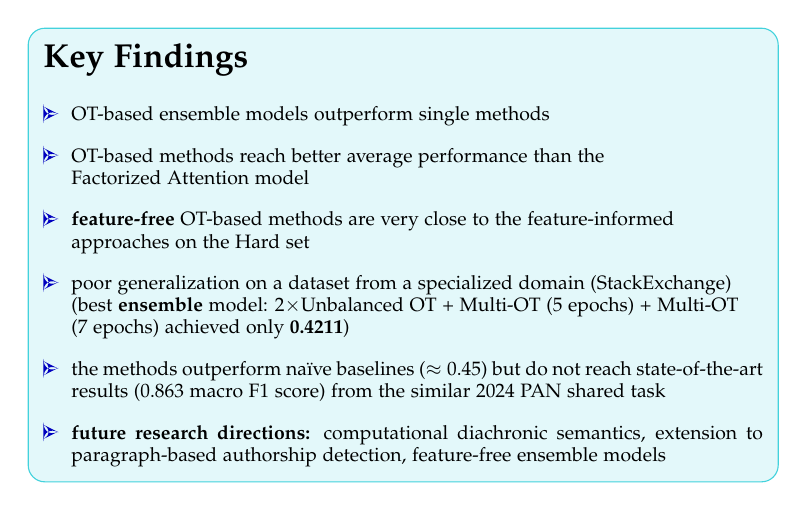
\begin{tikzpicture}
\node[
  draw=petrol!80,              
  fill=petrol!12,              
  rounded corners=6pt,
  minimum width=0.1\linewidth, 
  inner sep=5.5pt,               
  text width=0.8\linewidth-16pt, 
  font=\scriptsize,
  align=justify                
] (cap) {%
  \noindent \textbf{\large Key Findings}
  
\begin{itemize}[label=\bluebullet,left=0em,itemsep=3pt]
\item OT-based ensemble models outperform single methods
\item OT-based methods reach better average performance than the\\  Factorized Attention model
\item \textbf{feature-free} OT-based methods are very close to the feature-informed \\approaches on the Hard set
\item poor generalization on a dataset from a specialized domain (StackExchange)\\(best \textbf{ensemble} model:  2$\times$Unbalanced OT + Multi-OT (5 epochs) + Multi-OT\\(7 epochs) achieved only \textbf{0.4211})
\item the methods outperform na\"{i}ve baselines ($\approx 0.45$) but do not reach state-of-the-art results ($0.863$ macro F1 score) from the similar 2024 PAN shared task
\item \textbf{future research directions:} computational diachronic semantics, extension to paragraph-based authorship detection, feature-free ensemble models
\end{itemize}
  };
\end{tikzpicture}

\end{document}